\section{System Architecture}
\label{sec:design_sys_arch}

As described in \Cref{sec:analysis_deployment}, the \theResServer system is composed of two servers, the \acrfull{mks} and the \acrfull{prs}, serving two distinct purposes. The \acrshort{mks} creates private user keys with embedded attributes for all users. The \acrshort{prs} server stores and manages the distribution of the encrypted resources.

\Cref{sec:analysis_deployment} also describes the offline deployment of the \acrshort{mks} to provide implicit protection against external digital threats, and the public availability of the \acrshort{prs}. Further, \Cref{subsec:design_resources} describes the design decision to store metadata from resources on an internal database within the \acrshort{prs}, to offer details on the resources without exposing contents to the server.
\vskip 0.5em
The remaining piece of software in the \theResServer system is a Client tool for users to communicate with the \acrfull{prs} and to help with creation of policies. This \acrfull{crs} runs as a local web server on a user's device, allowing a user to emulate a direct connection to the \acrshort{prs}, wrapped in a simple \acrshort{html} user interface.

The \acrshort{crs} has direct access to a local \OpenABE library, to process encryption \& decryption operations (as well as key management) and uses \textit{some} Authentication Service to authenticate a user. The \acrshort{crs} also interfaces with the \acrshort{prs} to carry out the uploading \& downloading of resources for the user, as well as offering access to the \acrshort{prs}'s search functionality.
\vskip 0.5em
\begin{figure}[htp]
    \centering
    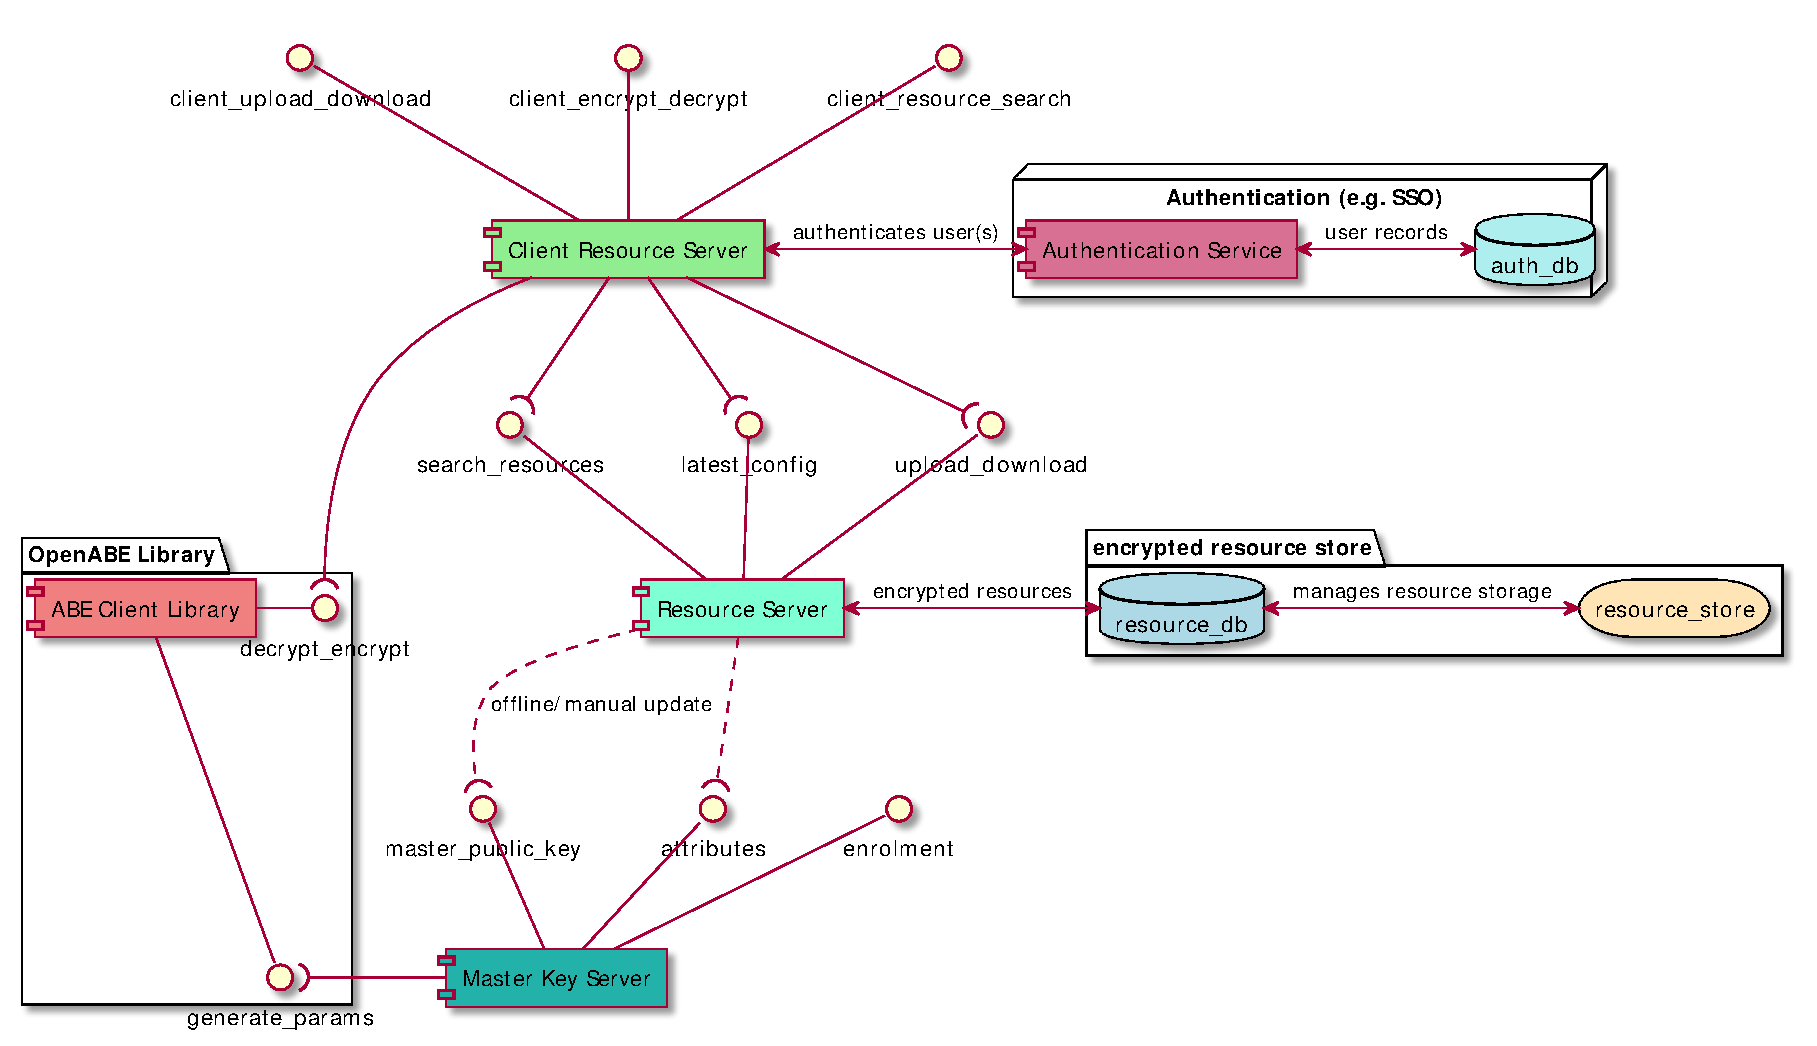
\includegraphics[width=\linewidth,keepaspectratio,]{images/infrastructure/system_architecture_abbrv.pdf}

    \caption{
      \label{fig:sys_arch_abbrv}
      A condensed system architecture diagram of the \theResServer system.
    }

\end{figure}
\Cref{fig:sys_arch_abbrv} represents the designed system architecture of the \theResServer system in a condensed form, with the full form presented in Appendix \ref{appendix:architecture_diagram}. As stated, the Authentication Service is left abstract in the design so that any organisation may identify and implement their own service. It should also be noted that in both design and diagram, the \acrshort{prs} does \textbf{not} have access to a copy of the \OpenABE library, ensuring it is unable to execute encryption or decryption tasks itself (as described in \Cref{subsec:analysis_deployment_prs}).
